\documentclass[a4paper]{article}
\usepackage[spanish]{babel}
\usepackage[utf8]{inputenc}
\usepackage{anysize}
\usepackage{setspace}
\usepackage{xcolor}
%\usepackage{float}
\usepackage[pdftex]{graphicx}
\usepackage{amsmath}
\usepackage[hypcap=true]{caption}
\usepackage[colorlinks, linkcolor= blue]{hyperref}



\begin{document}
\title{Dinámica del sólido rígido. Giróscopo}
\author{Álvaro Díaz Carmona}
%\date{Sesión del 7 de Diciembre de 2016}
\maketitle
\begin{abstract}
\url{https://github.com/adiaz97/paper}

En este informe se reproduce un experimento para analizar el movimiento de un sólido rígido. El objetivo principal es la determinación de uno de los momentos de inercia de este sólido y el estudio de su rotación, precesión y nutación.

\end{abstract}

\section{Introducción}
El movimiento giroscópico es el de un cuerpo que gira en torno a un eje móvil. En el caso concreto del giróscopo, el cuerpo tiene simetría de revolución y gran momento de inercia respecto al eje de giro. 
De la misma manera que la masa de un objeto está relacionada con su resistencia a cambiar su desplazamiento, el momento de inercia para un cierto sólido no es más que una magnitud que mide su resistencia a la rotación en cierto punto. Si el sólido tiene ciertas simetrías, el momento de inercia puede ser el mismo en varios puntos, en un eje o incluso en todo el sólido. El momento de inercia para cualquier sólido solo depende de la distribución de masa dentro del volumen que ocupa. Para su cálculo se puede usar su definición $I=\int^{M}_{0} r^2\mathrm{d}m$ donde $r$ es el módulo de la distancia al eje de rotación. Esta definición es válida cuando el eje de rotación del sólido coincide con alguno de los ejes principales (si existen) que son ejes perpendiculares entre sí y aportan información sobre simetrías del cuerpo. En general, puede haber desde 0 hasta 3 ejes de simetría distintos (llamados $X$, $Y$ y $Z$). 
También hay otra manera de conocer el momento de inercia para un sólido, aprovechando las simetrías y las leyes de la Mecánica. Por ejemplo, supongamos un disco circular con un cierto espesor, que puede hacerse girar sobre su eje de revolución a través de una polea que une el eje del disco con una masa libre para caer (ver \autoref{fig:disco1}).
\begin{figure}[h]
\begin{center}
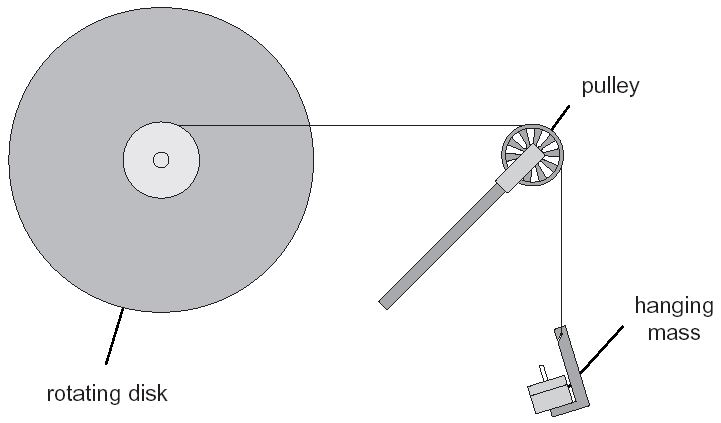
\includegraphics[width=10 cm]{disco1.png}
\caption{Disco y polea, según la disposición experimental.}
\label{fig:disco1}
\end{center}
\end{figure}
Podemos aplicar la segunda Ley de Newton en su versión angular:
\begin{equation}
\sum F=m_d a_d\equiv \sum M=I\alpha\,.
\end{equation}
Donde $\sum F$ es la suma de todas las fuerzas externas ejercidas sobre el disco, $m_d$ es su masa, $a_d$ es la aceleración lineal que adquiere, $\sum M$ es la suma de los momentos de las fuerzas externas  y $\alpha$ es la aceleración angular.
Sabemos que, al estar causando la rotación con la polea, se produce un movimiento de rodadura en el disco, entonces $\alpha=\frac{a}{R}$. Por otro lado, por la definición del momento de una fuerza tenemos que $\sum M=\vec{R}\times\vec{F}$ siendo $\vec{R}$ la distancia desde la fuerza al punto de aplicación. Así, pues, el momento de inercia en el eje de rotación (que es un eje principal del disco) es 
\begin{equation}
I=\frac{R^2\times F_{eje}}{a}\,.
\label{eq:inercia}
\end{equation}
Sucede que, en el eje, la única fuerza externa es la tensión de la cuerda $T$. El peso no contribuye porque su punto de aplicación (el centro de gravedad) está dentro del eje y por lo tanto su distancia es nula. Para averiguar la tensión volvemos a aplicar la segunda Ley de Newton, esta vez en su forma original:
\begin{equation}
\sum F=ma\Rightarrow mg-T=ma\Rightarrow T=m\left(g-a\right)\,.
\label{eq:tension}
\end{equation}
En este caso $m$ es la masa de la pesa, y $a$ es la aceleración lineal que tiene. Sustituyendo \eqref{eq:tension} en \eqref{eq:inercia} tenemos que 
\begin{equation}
I=mR^2\left(\frac{g}{a}-1\right)\,.
\label{eq:inerciadisco}
\end{equation}

De esta manera, observamos que cuanto mayor es la masa y el radio del disco mayor es el momento de inercia, esto es, más resistencia opone a girar si está en reposo o a dejar de girar si estaba en movimiento. También observamos que al aumentar la aceleración de la polea (el tirón de la cuerda) disminuye el momento de inercia.
Este sencillo cálculo servirá de base para la experiencia registrada en el informe, pero los conceptos son fácilmente generalizables a cualquier sólido rígido.
\section{Fundamento Teórico} \label{sec:fundamento}
Supóngase un sólido libre de girar sin rozamiento en torno a un punto fijo cuya velocidad angular inicial $\omega$ es constante y se encuentra en la parte positiva del eje $Z$. Su momento angular $\vec{L}$ quedará definido por:
\begin{equation}
\label{eq:defL}
\vec{L}=I_z \omega\, \hat{e}_{z}
\end{equation}
Siendo $I_z$ el momento de inercia respecto al eje $Z$ y $\hat{e}_{z}$ el vector unitario de ese mismo eje. En ausencia de momentos externos $\vec{M}_{ext}$	el momento angular no varía y se mantiene la dirección del eje de rotación. Matemáticamente
\begin{equation}
\frac{\mathrm{d}\vec{L}}{\mathrm{d}t}=\sum \vec{M}_{ext} =0\Leftrightarrow\vec{L}=cte\,.
\end{equation}
Si se cuelga un cuerpo de masa $m$ en un extremo del eje $Z$, se ejerce una fuerza peso $\vec{P}=m\vec{g}$ y, sabiendo que el momento de una fuerza es el producto vectorial de esta por el vector posición del punto de aplicación de la fuerza $\vec{r}\equiv d\hat{e}_z$, entonces obtenemos la siguiente ecuación: 
\begin{equation}
\label{eq:defdL}
\frac{\mathrm{d}\vec{L}}{\mathrm{d}t}=\vec{r}\times m\vec{g}\,.
\end{equation}
Esta fuerza aplicada causa que el eje de giro cambie de dirección y, por lo tanto, el cuerpo adquiere una velocidad angular perpendicular al eje $Z$. Si esta fuerza es muy pequeña y, teniendo en cuenta que $\omega=cte$, podemos escribir \eqref{eq:defdL} como 
\begin{equation}
\frac{\mathrm{d}\vec{L}}{\mathrm{d}t}=d\hat{e}_z\times m\vec{g}\approx I_z \omega\, \dot{\hat{e}}_{z}
\end{equation}
donde hemos hecho la derivada temporal en \eqref{eq:defL} despreciando la variación en el momento de inercia. De aquí podemos deducir que 
\begin{equation}
\label{eq:defOmega}
\dot{\hat{e}}_{z}=\vec{\Omega}\times \hat{e}_z\;\text{con}\,\vec{\Omega}\equiv -\frac{dmg}{I_z\omega}\hat{g}\,.
\end{equation}
Este fenómeno por el que el eje de rotación cambia de dirección se llama \textit{precesión} y la velocidad angular con la que rota, $\vec{\Omega}$, se llama velocidad angular de precesión.

\begin{figure}[h]
\begin{center}
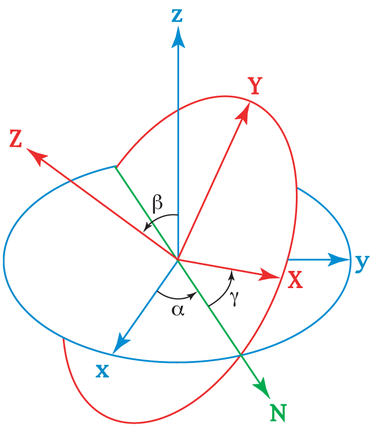
\includegraphics[width=8 cm]{euler.png}
\caption{Ángulos de Euler de un sólido cuyo \textcolor{red}{sistema de referencia propio} gira respecto al \textcolor{blue!70!cyan!85!white}{sistema de referencia del laboratorio} (azul)}
\label{fig:Euler}
\end{center}
\end{figure}

Hay otro fenómeno característico de un giróscopo, llamado \textit{nutación}. Conocidos los ángulos de Euler (ver \autoref{fig:Euler}), es fácil ver que la velocidad angular del sólido en torno a su eje es $\omega=\dot{\gamma}$ y $\dot{\alpha}$ corresponde a la precesión. Entonces, $\dot{\beta}$ representará un tercer movimiento al que hemos llamado nutación. Suponiendo la conservación de la energía, es demostrable que 
\begin{equation}
\label{eq:nutacion}
\dot{\beta}=\frac{A-B\cos\beta}{I_{12}\sin^2\beta}\, ,
\end{equation}
donde $A$ y $B$ son constantes y $I_{12}$ es el momento de inercia respecto a los ejes contenidos en el plano perpendicular al eje de rotación. Si $\beta$ adquiere un valor único habrá una precesión estacionaria; en cambio, si el ángulo oscila entre dos valores $\beta_a$ y $\beta_b$, podemos distinguir tres casos:
\begin{enumerate}
\item $\dot{\beta}$ nunca se anula, es decir, $\arccos\left(\frac{A}{B}\right)>\beta_b$ o $\arccos\left(\frac{A}{B}\right)<\beta_a$ . Entonces el eje precesa alrededor de la vertical (dirección $Z$) y su posición oscila periódicamente entre los ángulos. El movimiento proyectado es similar a una función seno o coseno.
\item Si $\beta_a<\arccos\left(\frac{A}{B}\right)<\beta_b$, el eje se mueve realizando bucles, $\dot{\beta}$ cambia de signo cuando el eje de rotación pasa de estar en la parte superior a la parte inferior del bucle.
\item En el caso límite $\arccos\left(\frac{A}{B}\right)=\beta_a$, el giróscopo oscila haciendo cúspides. El eje de rotación queda instantáneamente en reposo en la parte superior de cada cúspide.
\end{enumerate}
\section{Material y metodología} \label{sec:metodo}
Los materiales utilizados para esta demostración experimental son:
\begin{itemize}
\item Giróscopo Pasco ME 8960 (un disco plano capaz de girar en torno a su eje de revolución, ver \autoref{fig:pasco}).
\begin{figure}[h]
\begin{center}
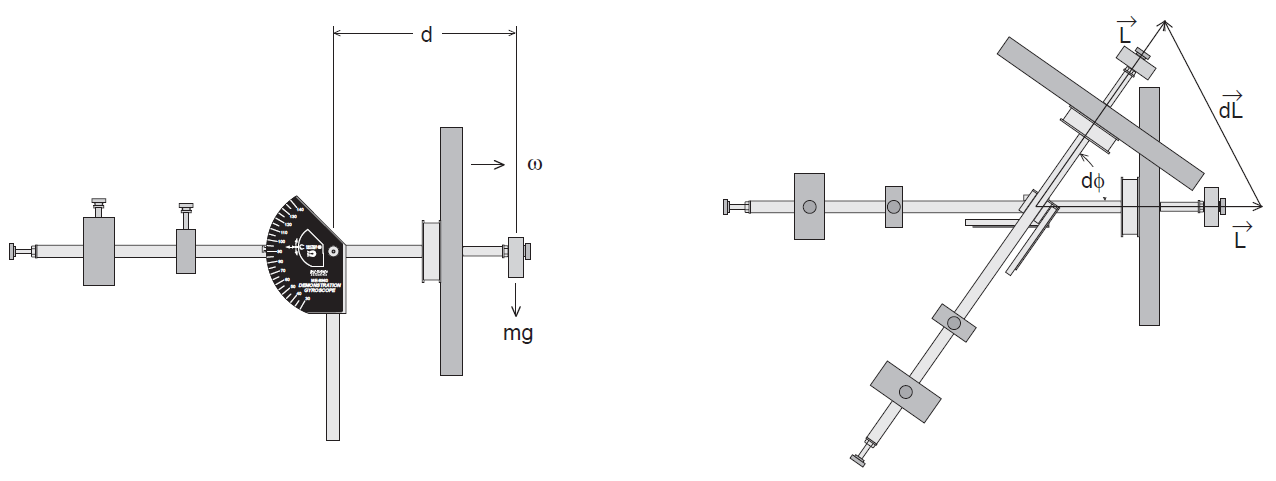
\includegraphics[width=12cm]{disco2.png}
\caption{Giróscopo utilizado en la experiencia.}
\label{fig:pasco}
\end{center}
\end{figure}
\item Pesas portátiles de diferentes masas.
\item Portapesas.
\item Polea.
\item Hilo.
\item Tres sensores.
\item Programas de DataStudio.
\end{itemize}
Para la determinación del momento de inercia del giróscopo se siguen los siguientes pasos, basados en el anterior \autoref{sec:fundamento}:
\begin{enumerate}
\item Colocar en un extremo del hilo el portapesas con pesas medidas anteriormente. Pasar el hilo por la polea y unirlo al giróscopo.
\item Liberar el portapesas para que caiga mueva la polea. Recoger datos de la aceleración del disco con el ordenador. 
\item Repetir el proceso hasta tomar las medidas necesarias.
\end{enumerate}
Para la determinación de la velocidad angular de precesión se siguen los siguientes pasos:
\begin{enumerate}
\item Equilibrar el giróscopo.
\item Colocar una masa ya medida en el extremo del giróscopo. Anotar la distancia $d$ entre la masa y el eje de giro.
\item Quitar la pesa utilizada. Abrir el programa de DataStudio y, sujetando el eje del giroscopio poner en marcha el aparato utilizando el hilo para dar impulso. La eficiencia de la toma de datos aumenta cuanto mayor sea la velocidad proporcionada.
\item Con ayuda del sensor, determinar la velocidad angular de rotación.
\item Mientras el disco gira, colocar la pesa en la posición indicada y, con ayuda del otro sensor, medir la velocidad angular de precesión.
\item Una vez medida, soltar el eje de rotación y quitar la pesa. Volver a medir la velocidad de rotación. 
\item Repetir el proceso haciendo girar el disco en sentido contrario.
\end{enumerate}
Finalmente, para la determinación de la velocidad angular de nutación se siguen los siguientes pasos:
\begin{enumerate}
\item Abrir el tercer programa de DataStudio y colocar el eje del disco formando 30º con la horizontal.
\item Determinar la velocidad angular de rotación (al principio y al final del ensayo), de precesión y de nutación con ayuda de los sensores.
\item Repetir el paso 2 pero empujando suavemente el eje del disco en la dirección de la precesión. Anotar el movimiento observado.
\item Repetir el paso 2 pero ahora empujando en sentido contrario.
\end{enumerate}
\section{Datos recogidos}
En primer lugar se tomaron medidas de los parámetros básicos para el ensayo (ver \autoref{tab:radios}). También se midieron las masas disponibles (ver \autoref{tab:masas}).
\begin{table}[h]
\begin{center}
\begin{tabular}{|c|c|c|}
\cline{2-3}
\multicolumn{1}{c|}{}& Radio & Espesor\\
\hline
Disco&$\left(12,7\pm 0,1\right)\times 10^{-2}\,\text{m}$&$\left(2,1\pm 0,1\right)\times 10^{-2}\,\text{m}$\\
\hline
Polea&$\left(2,3\pm 0,1\right)\times 10^{-2}\,\text{m}$&\multicolumn{1}{c}{}\\
\cline{1-2}
\end{tabular}
\caption{Parámetros del disco y la polea}
\label{tab:radios}
\end{center}
\end{table}
\begin{table}[h]
\begin{center}
\begin{tabular}{|c|c|}
\cline{2-2}
\multicolumn{1}{c|}{}&$\left( \text{Masa}\pm 0,1\right) \times 10^{-3}\,\text{kg}$\\ \hline
$m_1$&$101,6$\\ \hline
$m_2$&$132,1$\\ \hline
$m_3$&$71,0$\\ \hline
$m_4$&$40,4$\\ \hline
$m_5$&$162,4$\\ \hline
\end{tabular}
\caption{Masas utilizadas en la primera parte}
\label{tab:masas}
\end{center}
\end{table}
Para la segunda y tercera parte de esta experiencia, se usa una masa $m=\left(152,6\pm 0,1\right)\times 10^{-3} \text{kg}$. El parámetro $d$ utilizado en la ecuación \eqref{eq:defOmega} es $d=\left(32,0\pm 0,1\right)\times 10^{-2} \text{m}$. 

Durante la observación de la nutación se recogieron gráficas en cada ensayo, similares a la \autoref{fig:nuta1}
\begin{figure}[h]
\begin{center}
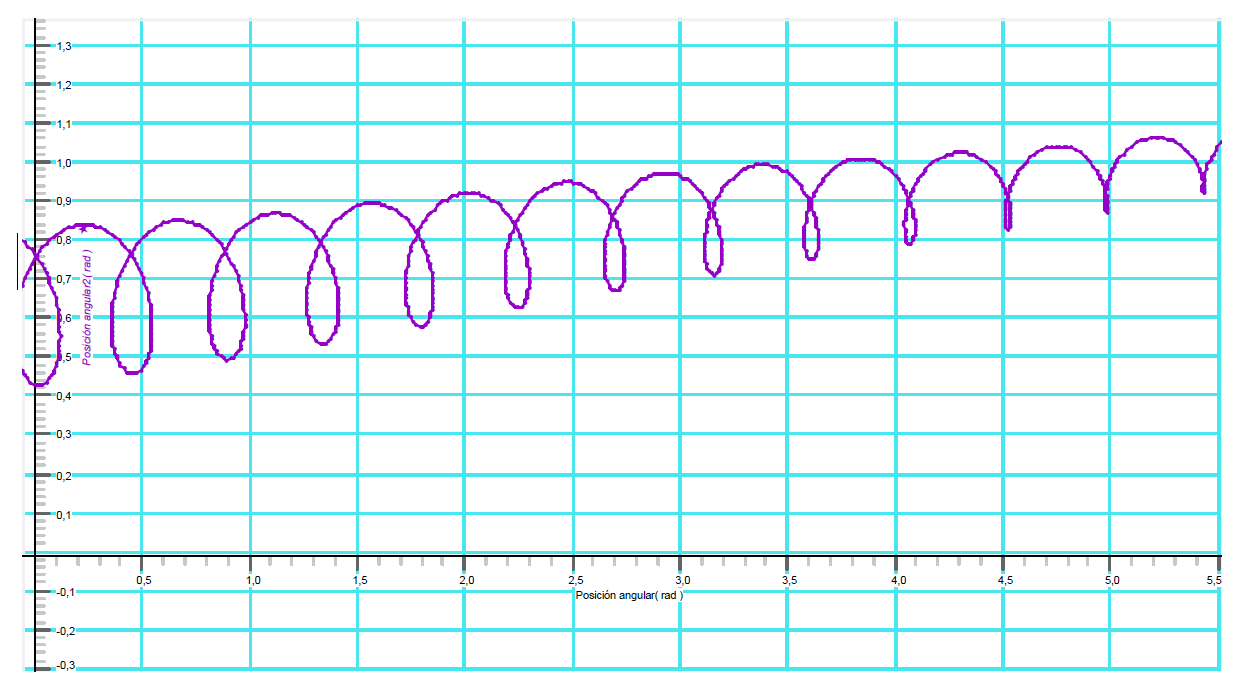
\includegraphics[width=12 cm]{nuta1.png}
\caption{Observación representativa del fenómeno de la nutación.}
\label{fig:nuta1}
\end{center}
\end{figure}
\section{Resultados} \label{sec:resultados}
Siguiendo la metodología \ref{sec:metodo} citada, se realizaron varios ensayos para calcular el momento de inercia del giróscopo. Es demostrable que, para una disposición como la indicada, podemos obtener el momento de inercia a partir de la aceleración $\vec{a}$ de la pesa que cae (\autoref{eq:inercia}). Los resultados conseguidos se recogen en la \autoref{tab:inercia}.
\begin{table}[h]
\begin{center}
\begin{tabular}{|c|c|c|c|}
\hline
Ensayo & Aceleración $\left(\text{m/s}^2\right)$ & Masa $\left(\pm 0,0001\,\text{kg}\right)$ & Momento de inercia $\left(\text{kg/m}^2\right)$\\
\hline
1 & $0,06220\pm 0,00024$ & $0,1016$ & $0,842\pm 0,008$\\
\hline
2 & $0,0817\pm 0,0005$ & $0,1321$ & $0,832\pm 0,009$\\
\hline
3 & $0,0431\pm 0,0004$ & $0,0710$ & $0,851\pm 0,010$\\
\hline
4 & $0,02380\pm 0,00016$ & $0,0405$ & $0,881\pm 0,010$\\
\hline
5 & $0,1030\pm 0,0005$ & $0,1624$ & $0,809\pm 0,008$\\
\hline
Promedio & $0,0628\pm 0,0004$ & $0,1015$ & $0,843\pm 0,009$\\
\hline
\end{tabular}
\caption{Datos y resultados para el momento de inercia.}
\label{tab:inercia}
\end{center}
\end{table}
Luego el momento de inercia del disco es 
\begin{equation}
I_z=0,843\pm 0,009\,\text{kg/m}^2\,.
\end{equation}
En la segunda parte de la demostración, se midieron la velocidad angular inicial $\omega_1$, la velocidad angular de precesión $\vec{\Omega}_{exp}$ y la velocidad angular inicial $\omega_2$. También se calculó el valor teórico para la velocidad de precesión $\vec{\Omega}_{teo}$ usando la expresión \eqref{eq:defOmega}. Los resultados para los distintos ensayos están en la tabla \autoref{tab:precesion}.
\begin{table}[h]
\begin{center}
\begin{tabular}{|c|c|c|c|c|}
\hline
Ensayo & $\omega_1\,\left(\pm 0,001\,\text{rad/s}\right)$ & $\vec{\Omega}_{exp}\,\left(\text{rad/s}\right)$ & $\omega_2\,\left(\pm 0,001\,\text{rad/s}\right)$ & $\vec{\Omega}_{teo}\,\left(\text{rad/s}\right)$ \\
\hline
1 & $57,461$ & $0,4178\pm 0,0004\,\vec{g}$ & $49,099$ & $0,421\pm 0,005\,\vec{g}$ \\
\hline
2 & $45,397$ & $0,507\pm 0,001\,\vec{g}$ & $38,811$ & $0,526\pm 0,006\,\vec{g}$ \\
\hline1 & $49,943$ & $0,4620\pm 0,0006\,\vec{g}$ & $44,999$ & $0,472\pm 0,005\,\vec{g}$ \\
\hline
\end{tabular}
\caption{Datos recogidos y resultados para la velocidad angular de precesión}
\label{tab:precesion}
\end{center}
\end{table}
Finalmente, en el estudio del movimiento de nutación se realizaron varios ensayos siguiendo la metodología en la \autoref{sec:metodo}. En casi todos los ensayos se observó que el eje del disco describía bucles (Caso 2) salvo en uno solo, donde se registró una trayectoria con cúspides (Caso 3). A continuación se muestran dos ejemplos de las gráficas recogidas en las Figuras \ref{fig:nuta2} y \ref{fig:nuta3}.
\begin{figure}[h]
\begin{center}
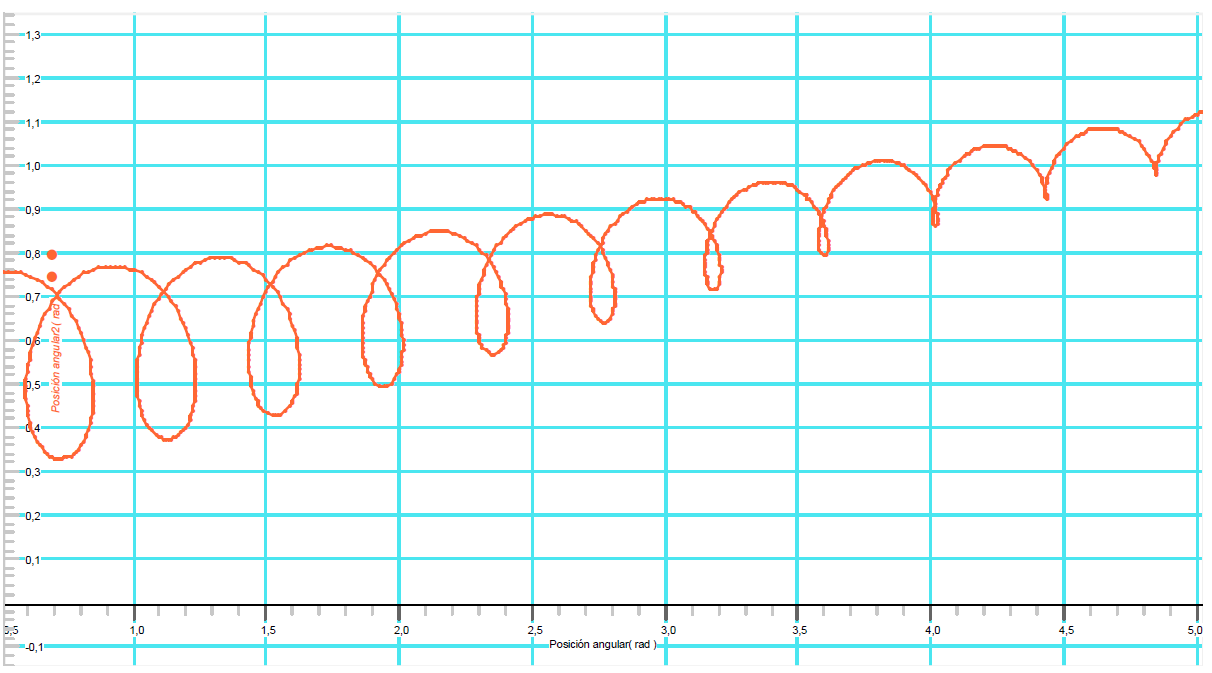
\includegraphics[width=12 cm]{nuta2.png}
\caption{Observación del segundo caso de nutación.}
\label{fig:nuta2}
\end{center}
\end{figure}
\begin{figure}[h]
\begin{center}
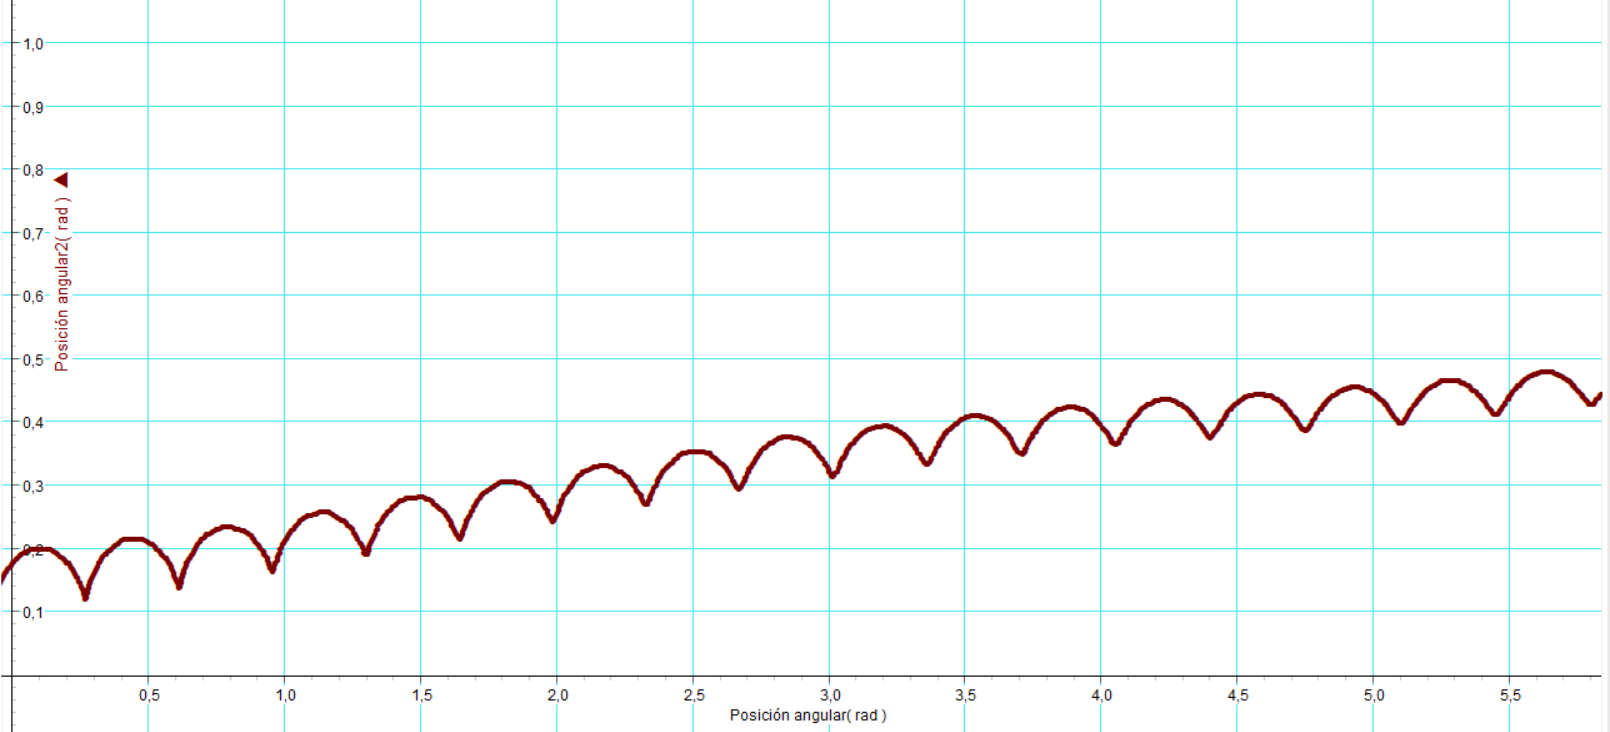
\includegraphics[width=12 cm]{nuta3.png}
\caption{Observación del tercer caso de nutación.}
\label{fig:nuta3}
\end{center}
\end{figure}
\section{Conclusiones}
Siguiendo los pasos descritos se calculó el momento de inercia a partir de medidas de la aceleración y se obtuvo el resultado final de $I_z=0,843\pm 0,009\,\text{kg/m}^2$ con una dispersión de $\sigma=0,022\,\text{kg/m}^2$. Este valor de dispersión significa que los valores obtenidos son próximos, luego las medidas y los cálculos se realizaron con precisión.

Respecto a la determinación de la velocidad angular de precesión, la comparación entre los valores medidos y los cálculos en la \autoref{tab:Omega} arroja errores relativos en los módulos menores al 2\% para todos los casos, mientras que la dirección y sentido coinciden. Así pues estos cálculos tienen exactitud y precisión. También es importante notar que, comparando la velocidad angular inicial y final de rotación, observamos que el disco es efectivamente frenado, es decir, $\omega$ no es estrictamente constante. Atribuimos este hecho a rozamientos entre el disco y su eje de giro.

\begin{table}[h]
\begin{center}
\begin{tabular}{|c|c|c|}
\hline
$\Omega_{exp}\,\left(\text{rad/s}\right)$ & $\Omega_{teo}\,\left(\text{rad/s}\right)$ & Error relativo (\%)\\
\hline
$0,4178\pm 0,0004$ & $0,421\pm 0,005$ & 0,29 \\
\hline
$0,507\pm 0,001$ & $0,526\pm 0,006$ & 1,94\\
\hline
$0,4620\pm 0,0006$ & $0,472\pm 0,005$ & 1,04\\
\hline
\end{tabular}
\caption{Comparación de los módulos de las velocidades de precesión experimentales y teóricas}
\label{tab:Omega}
\end{center}
\end{table}

Finalmente, se observaron los movimientos de nutación descritos en la  \eqref{sec:resultados} y se descubrió que en las condiciones del laboratorio había preferencia por el caso 2 de nutación (bucles), salvando una excepción en la que se observó el caso 3 (cúspides). Además se comprobó cualitativamente que el cabeceo o nutación se reduce si se empuja el eje del giroscopio en sentido de la precesión y, recíprocamente, al aplicar una fuerza externa en sentido opuesto al movimiento de precesión, el cabeceo se acrecenta.
\section*{Apéndices}
\subsection*{Apéndice de errores}
\begin{itemize}
\item Momento de inercia.
\begin{equation}
\Delta I_z=\sqrt{\left(R^2\left(\frac{g}{a}-1\right)\right)^2\left(\Delta m\right)^2+\left(2m\left(\frac{g}{a}-1\right)\right)^2 \left(\Delta R\right)^2+\left(mR^2\left(\frac{g}{a^2}\right)\right)^2\left(\Delta a\right)^2}
\end{equation}
\item Velocidad angular de precesión.
\begin{equation}
\Delta\Omega_{teo}=\sqrt{\left(\frac{mg}{I_z\omega_{rot}}\right)^2\left(\Delta d\right)^2+\left(\frac{dmg}{I_z\omega_{rot}}\right)^2\left(\Delta m\right)^2+\left(\frac{dmg}{I^2_z\omega_{rot}}\right)^2 \left(\Delta I_z\right)^2+\left(\frac{dmg}{I_z \omega^2_{rot}}\right)^2\left(\Delta \omega_{rot}\right)^2}
\end{equation}

\end{itemize}
\nocite{*}
\bibliographystyle{unsrt}
\bibliography{mecanica.bib}
\end{document}


